\section{Results}
\begin{figure*}[t]
    \centering
    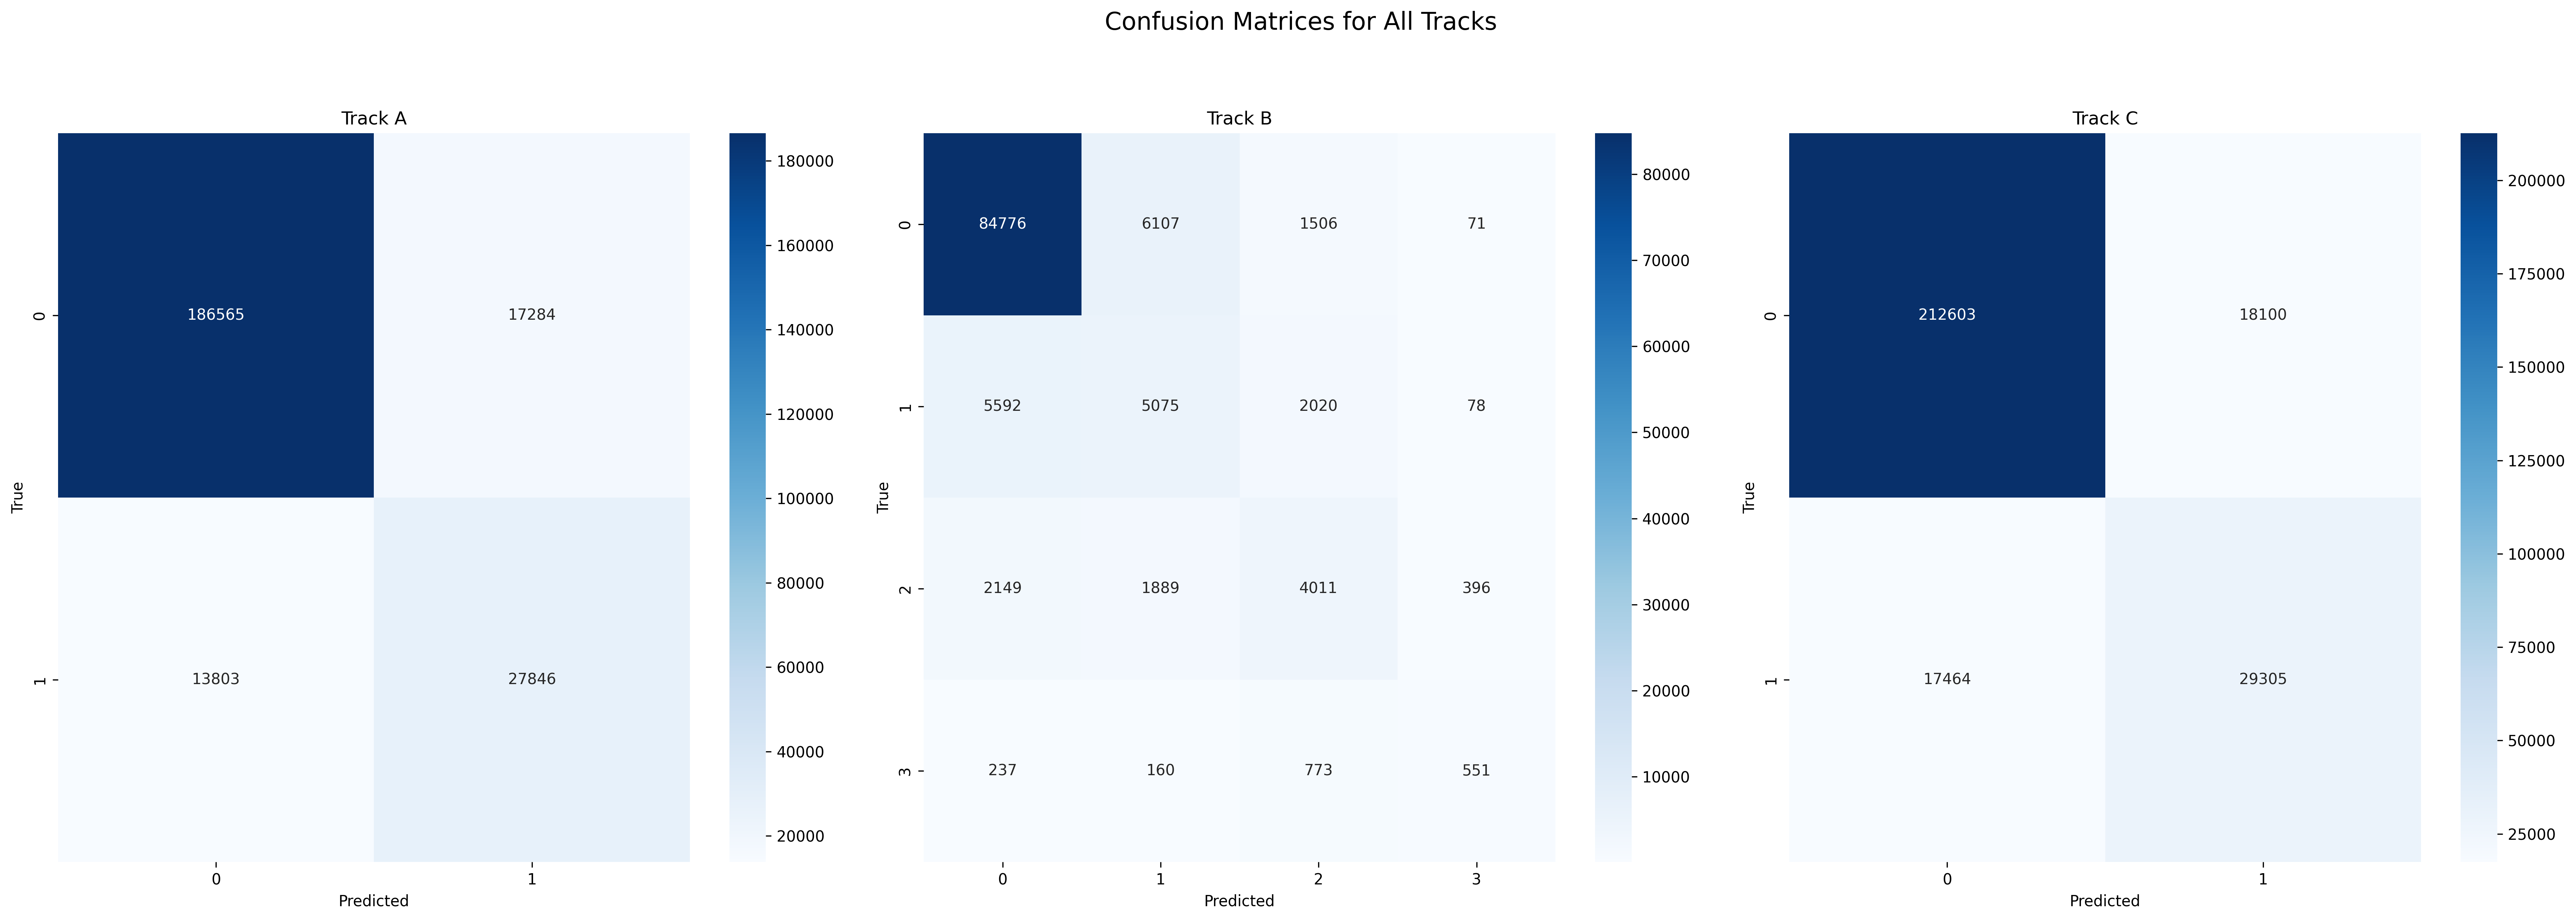
\includegraphics[width=1.7\columnwidth]{images/confusion_matrices_all_tracks.png}
    \caption{Confusion matrices for each language across Tracks A, B, and C.}
    \label{fig:confusion_matrices}
\end{figure*}
Extensive experiments were conducted on multiple models to determine the most effective approach for multi-label emotion detection across various languages. The selected model was trained on datasets corresponding to each language, and its performance was analyzed using the test dataset. The evaluation results are presented in Table \ref{tab:results}. More detailed results and additional analysis can be found in the Appendix \ref{sec:appendix_model_selection}.

Additionally, in specific languages such as Tigrinya and Kinyarwanda in Track-C, our approach secured the second rank in the competition. This success can be attributed to the integration of innovative preprocessing steps and using language-specific model embeddings.
% Furthermore, converting emojis into their corresponding textual representations had a positive impact on performance, particularly in languages where emojis commonly appear in social media text.

A comparison of our findings with reference studies \cite{muhammad2025brighterbridginggaphumanannotated} highlights the effectiveness of our approach. By leveraging domain-specific model embeddings, our models were able to bridge the gap in emotion classification for low-resource languages.

Figure \ref{fig:confusion_matrices} presents the pooled confusion matrices for Tracks A, B, and C. For Track A, the binary matrix shows 186565 true negatives, 17284 false positives, 13803 false negatives, and 27846 true positives, indicating strong classification performance with some misclassification at the decision boundaries. The four-class matrix for Track B highlights misclassifications among intermediate intensity levels, while the binary matrix for Track C, with 212603 true negatives and 29305 true positives, reveals a balanced yet imperfect performance in cross-lingual detection.

% \begin{figure}[h]
%     \centering
%     \includegraphics[width=\linewidth]{performance_plot.png} % Replace with actual figure filename
%     \caption{Performance of the best models based on the F1-score metric. The ranking of results for each language is compared with other participants and the best participant’s accuracy. Reference articles \cite{muhammad2025brighterbridginggaphumanannotated} were used to benchmark our results.}
%     \label{table:1}
% \end{figure}
% % lang:my_model rank/all best_model base_line
% TrackA:
% afr:54.01 15/37 69.86
% amh:61.20 19/43 77.31
% arq:51.07 24/43 66.87
% ary:51.88 20/41 62.92
% chn:56.65 30/41 70.94
% deu:60.60 25/50 73.99
% eng:73.97 35/96 82.30
% esp:76.19 26/47 84.88
% hau:63.22 18/40 75.07
% hin:80.32 33/43 92.57
% ibo:50.93 14/34 60.01
% ind:-
% jav:-
% kin:51.94 6/31 65.74
% mar:81.10 23/42 90.58
% orm:54.31 11/36 61.64
% pcm:53.09 22/34 67.40
% ptbr:47.99 27/42 68.33
% ptmz:50.08 6/36 54.77
% ron:73.75 14/43 79.43
% rus:82.42 33/50 90.87
% som:48.26 10/34 57.65
% sun:42.48 19/37 54.97
% swa:29.52 15/32 41.47
% swe:56.51 13/40 62.62
% tat:64.32 18/36 84.59
% tir:52.37 6/34 59.05
% ukr:48.62 29/40 72.56
% vmw:16.815/31 32.50
% xho:-
% yor:34.09 9/32 46.13
% zul:-
% TrackB:
% afr:-
% amh:49.42 14/23 85.58 -
% arq:36.54 18/26 63.38 36.37
% ary:-
% chn:48.47 19/27 72.24 51.86
% deu:54.10 18/27 76.57 56.21
% eng:68.81 28/43 84.04 64.15
% esp:66.70 23/29 80.80 72.59
% hau:58.42 15/26 77.00 39.16
% hin:-
% ibo:-
% ind:-
% jav:-
% kin:-
% mar:-
% orm:-
% pcm:-
% ptbr:38.20 22/25 71.00 46.72
% ptmz:-
% ron:57.61 19/26 72.60 57.69
% rus:78.41 22/30 92.54 87.66
% som:-
% sun:-
% swa:-
% swe:-
% tat:-
% tir:-
% ukr:42.55 17/24 70.75 43.54
% vmw:-
% xho:-
% yor:-
% zul:-
% TrackC:
% afr:54.01 4/14 70.50 61.28
% amh:61.20 6/13 66.68 -
% arq:51.07 6/14 65.35 55.75
% ary:51.88 6/12 63.22 52.76
% chn:56.65 7/15 56.65 55.23
% deu:60.60 6/15 73.62 59.17
% eng:73.97 4/17 82.07 65.58
% esp:76.19 5/15 85.00 73.29
% hau:63.22 4/13 73.14 51.91
% hin:80.32 6/16 92.16 79.73
% ibo:50.93 4/12 60.47 37.40
% ind:35.64 15/17 67.24 57.29
% jav:25.62 12/13 25.62 50.47
% kin:51.94 2/11 64.59 34.36
% mar:81.10 6/13 90.42 77.24
% orm:54.31 3/11 60.07 -
% pcm:53.09 5/10 67.40 48.67
% ptbr:47.99 8/14 68.36 51.60
% ptmz:50.08 3/14 55.54 40.44
% ron:73.75 4/15 77.27 76.23
% rus:82.42 6/17 90.62 76.97
% som:48.26 4/13 56.66 -
% sun:42.48 4/11 50.72 46.33
% swa:29.52 5/14 38.43 33.27
% swe:56.51 6/13 64.53 51.18
% tat:64.32 5/11 83.59 60.66
% tir:52.37 2/10 55.24 -
% ukr:48.62 10/17 71.99 54.76
% vmw:16.80 6/9 26.02 20.41
% xho:16.64 6/10 44.26 30.79
% yor:34.09 4/11 46.79 27.44
% zul:16.35 8/11 16.35 22.03
% \begin{table}[ht]
% \centering
% \caption{Results for each language across Tracks A, B, and C. The columns show the F1 macro scores for the proposed model (My Model), the best model from the literature (Best Model), the dataset paper reference (Paper/Dataset) where applicable, and the rank of the proposed model among all participants (My Rank).}
% \label{tab:results}
% \small
% \setlength{\tabcolsep}{4pt} % Adjust spacing
% \begin{tabular}{@{} l *{3}{D{.}{.}{2.2} d} *{4}{D{.}{.}{2.2} d} *{4}{D{.}{.}{2.2} d} @{}}
% \toprule
% \multirow{2}{*}{Lang} & 
% \multicolumn{3}{c}{Track A} & 
% \multicolumn{4}{c}{Track B} & 
% \multicolumn{4}{c}{Track C} \\
% \cmidrule(lr){2-4} \cmidrule(lr){5-8} \cmidrule(lr){9-12}
%  & \text{My Model} & \text{Best Model} & \text{Rank} 
%  & \text{My Model} & \text{Best Model} & \text{Paper/Dataset} & \text{Rank} 
%  & \text{My Model} & \text{Best Model} & \text{Paper/Dataset} & \text{Rank} \\
%  \midrule
%  afr & 54.01 & 69.86 & 15/37 & — & — & — & — & 54.01 & 70.50 & 61.28 & 4/14 \\
%  amh & 61.20 & 77.31 & 19/43 & 49.42 & 85.58 & — & 14/23 & 61.20 & 66.68 & — & 6/13 \\
%  arq & 51.07 & 66.87 & 24/43 & 36.54 & 63.38 & 36.37 & 18/26 & 51.07 & 65.35 & 55.75 & 6/14 \\
%  ary & 51.88 & 62.92 & 20/41 & — & — & — & — & 51.88 & 63.22 & 52.76 & 6/12 \\
%  chn & 56.65 & 70.94 & 30/41 & 48.47 & 72.24 & 51.86 & 19/27 & 56.65 & 56.65 & 55.23 & 7/15 \\
%  deu & 60.60 & 73.99 & 25/50 & 54.10 & 76.57 & 56.21 & 18/27 & 60.60 & 73.62 & 59.17 & 6/15 \\
%  eng & 73.97 & 82.30 & 35/96 & 68.81 & 84.04 & 64.15 & 28/43 & 73.97 & 82.07 & 65.58 & 4/17 \\
%  esp & 76.19 & 84.88 & 26/47 & 66.70 & 80.80 & 72.59 & 23/29 & 76.19 & 85.00 & 73.29 & 5/15 \\
%  hau & 63.22 & 75.07 & 18/40 & 58.42 & 77.00 & 39.16 & 15/26 & 63.22 & 73.14 & 51.91 & 4/13 \\
%  hin & 80.32 & 92.57 & 33/43 & — & — & — & — & 80.32 & 92.16 & 79.73 & 6/16 \\
%  ibo & 50.93 & 60.01 & 14/34 & — & — & — & — & 50.93 & 60.47 & 37.40 & 4/12 \\
%  ind & — & — & — & — & — & — & — & 35.64 & 67.24 & 57.29 & 15/17 \\
%  jav & — & — & — & — & — & — & — & 25.62 & 25.62 & 50.47 & 12/13 \\
%  kin & 51.94 & 65.74 & 6/31 & — & — & — & — & 51.94 & 64.59 & 34.36 & 2/11 \\
%  mar & 81.10 & 90.58 & 23/42 & — & — & — & — & 81.10 & 90.42 & 77.24 & 6/13 \\
%  orm & 54.31 & 61.64 & 11/36 & — & — & — & — & 54.31 & 60.07 & — & 3/11 \\
%  pcm & 53.09 & 67.40 & 22/34 & — & — & — & — & 53.09 & 67.40 & 48.67 & 5/10 \\
%  ptbr & 47.99 & 68.33 & 27/42 & 38.20 & 71.00 & 46.72 & 22/25 & 47.99 & 68.36 & 51.60 & 8/14 \\
%  ptmz & 50.08 & 54.77 & 6/36 & — & — & — & — & 50.08 & 55.54 & 40.44 & 3/14 \\
%  ron & 73.75 & 79.43 & 14/43 & 57.61 & 72.60 & 57.69 & 19/26 & 73.75 & 77.27 & 76.23 & 4/15 \\
%  rus & 82.42 & 90.87 & 33/50 & 78.41 & 92.54 & 87.66 & 22/30 & 82.42 & 90.62 & 76.97 & 6/17 \\
%  som & 48.26 & 57.65 & 10/34 & — & — & — & — & 48.26 & 56.66 & — & 4/13 \\
%  sun & 42.48 & 54.97 & 19/37 & — & — & — & — & 42.48 & 50.72 & 46.33 & 4/11 \\
%  swa & 29.52 & 41.47 & 15/32 & — & — & — & — & 29.52 & 38.43 & 33.27 & 5/14 \\
%  swe & 56.51 & 62.62 & 13/40 & — & — & — & — & 56.51 & 64.53 & 51.18 & 6/13 \\
%  tat & 64.32 & 84.59 & 18/36 & — & — & — & — & 64.32 & 83.59 & 60.66 & 5/11 \\
%  tir & 52.37 & 59.05 & 6/34 & — & — & — & — & 52.37 & 55.24 & — & 2/10 \\
%  ukr & 48.62 & 72.56 & 29/40 & 42.55 & 70.75 & 43.54 & 17/24 & 48.62 & 71.99 & 54.76 & 10/17 \\
%  vmw & 16.81 & 32.50 & 5/31 & — & — & — & — & 16.80 & 26.02 & 20.41 & 6/9 \\
%  xho & — & — & — & — & — & — & — & 16.64 & 44.26 & 30.79 & 6/10 \\
%  yor & 34.09 & 46.13 & 9/32 & — & — & — & — & 34.09 & 46.79 & 27.44 & 4/11 \\
%  zul & — & — & — & — & — & — & — & 16.35 & 16.35 & 22.03 & 8/11 \\
%  \bottomrule
% \end{tabular}
% \end{table}
